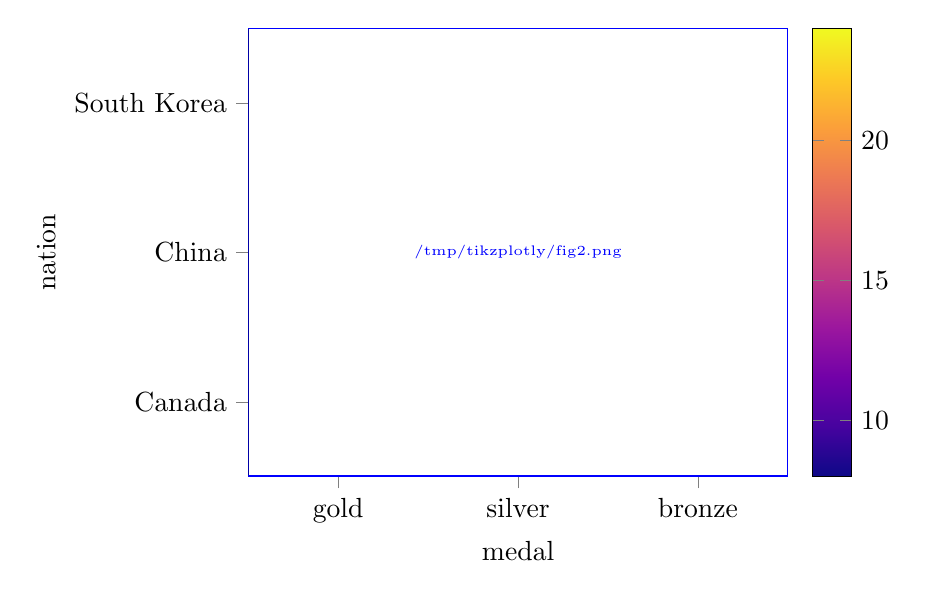
\begin{tikzpicture}


\begin{axis}[
y dir=reverse,
colorbar,
xtick={0,1,2},
xticklabels={gold,silver,bronze},
ytick={0,1,2},
yticklabels={South Korea,China,Canada},
colormap={mycolor}{
rgb255(0.0cm)=(13,8,135);
rgb255(0.1111111111111111cm)=(70,3,159);
rgb255(0.2222222222222222cm)=(114,1,168);
rgb255(0.3333333333333333cm)=(156,23,158);
rgb255(0.4444444444444444cm)=(189,55,134);
rgb255(0.5555555555555556cm)=(216,87,107);
rgb255(0.6666666666666666cm)=(237,121,83);
rgb255(0.7777777777777778cm)=(251,159,58);
rgb255(0.8888888888888888cm)=(253,202,38);
rgb255(1.0cm)=(240,249,33);
},
point meta max=24.0,
point meta min=8.0,
xmin=-0.5,
xmax=2.5,
ymin=-0.5,
ymax=2.5,
tick align=outside,
tick pos=left,
xlabel=medal,
ylabel=nation
]
\addplot+ graphics[includegraphics cmd=\pgfimage,xmin=-0.5, xmax=2.5, ymin=2.5, ymax=-0.5] {/tmp/tikzplotly/fig2.png};
\end{axis}
\end{tikzpicture}
